\chapter{Classification and regression trees}
\label{ch:decision-trees}

\begin{learningobjectives}
After this chapter, you should be able to:
\begin{itemize}
  \item interpret a tree as a recursive partition and a piecewise-constant
  prediction rule;
  \item derive classification impurity and regression squared-error reduction;
  \item explain greedy split search, structural constraints, and
  cost-complexity pruning;
  \item design leakage-safe classification and regression evaluations;
  \item audit instability, threshold, extrapolation, missingness, and
  interpretation failures; and
  \item separate an applied notebook from reusable package code and executable
  behavior contracts.
\end{itemize}
\end{learningobjectives}

\begin{chapterconnection}
Nearest neighbors let nearby observations vote or average. A decision tree
learns the neighborhood itself: a sequence of binary questions creates
axis-aligned regions, and each terminal region returns a class distribution or
a response mean. This representation captures nonlinearities and interactions
without feature scaling. Its greedy construction is also unstable. That
instability motivates the ensembles in the next chapter.
\end{chapterconnection}

\section{From questions to a prediction function}

An internal node asks whether feature $x_j$ is at most threshold $t$. The
answer routes an observation left or right. Repeating this operation partitions
feature space into disjoint rectangular regions $R_1,\dots,R_M$. The resulting
predictor has the form
\[
  \widehat f(x)=\sum_{m=1}^{M}c_m\,\mathbf 1\{x\in R_m\},
\]
where $c_m$ is a class decision, a class-probability vector, or a numerical
response. The model is piecewise constant: inputs can move within a leaf
without changing the prediction, then cross one threshold and jump abruptly.

Figure~\ref{fig:tree-partition} shows how a root question and two child
questions create four possible regions. The tree diagram and the feature-space
partition are two views of the same mathematical object.

\begin{figure}[htbp]
  \centering
  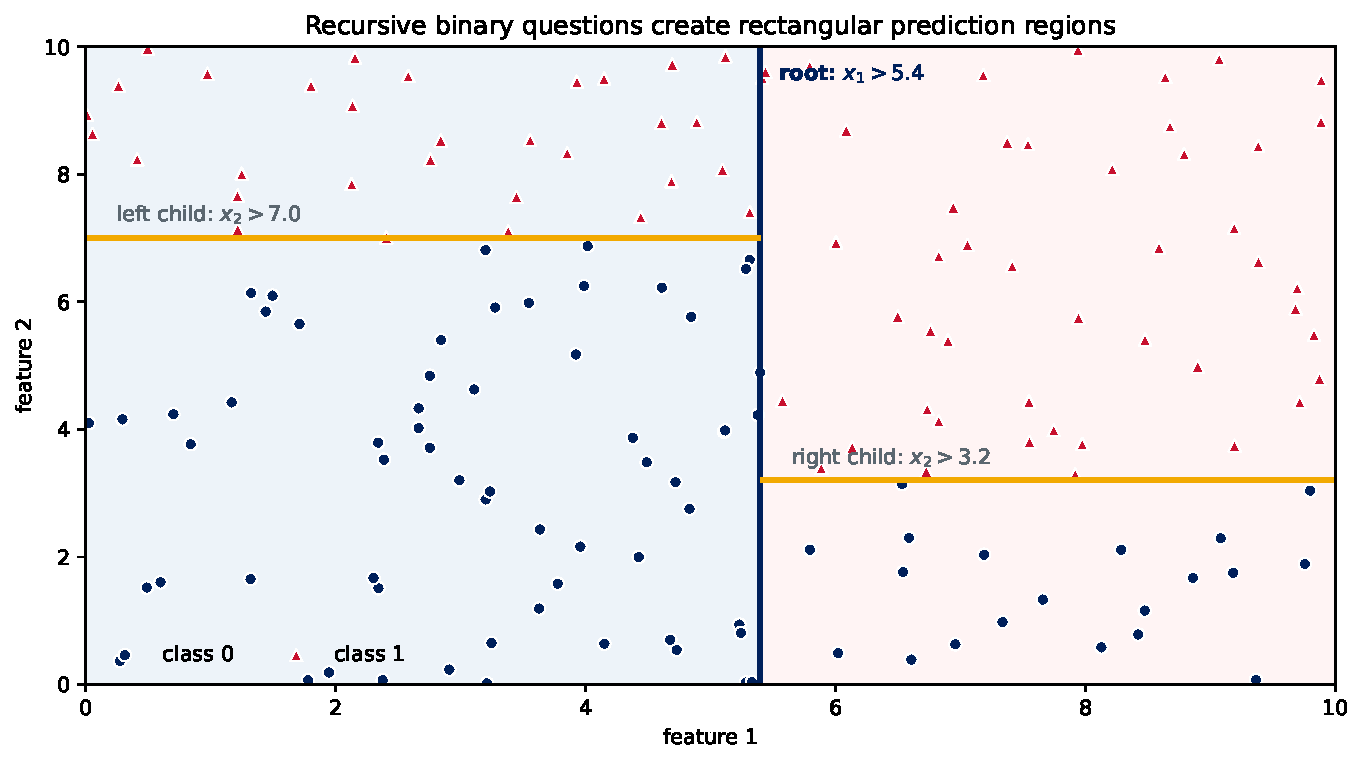
\includegraphics[width=0.92\textwidth]{figures/generated/tree-recursive-partition.pdf}
  \caption{Recursive binary questions create axis-aligned regions. The root
  split extends across the full domain; each child split applies only inside
  the region inherited from its parent.}
  \label{fig:tree-partition}
\end{figure}

The representation is locally interpretable in a narrow sense. A root-to-leaf
path exactly states which conditions in this fitted artifact produced an
output. It does not identify a biological mechanism, a causal effect, or a
stable population law.

\section{Classification trees estimate local class distributions}

Suppose node $S$ contains $n$ observations from $K$ classes. Let
$n_k$ be the class-$k$ count and $p_k=n_k/n$. Two common impurity measures are
\[
  G(S)=1-\sum_{k=1}^{K}p_k^2,
  \qquad
  H(S)=-\sum_{k:p_k>0}p_k\log_2 p_k.
\]
Gini impurity is zero for a pure node and largest when class mass is evenly
distributed. To see why it is meaningful, draw two labels $Y$ and $Y'$ independently
from the node proportions. Then
\[
  \Pr(Y\ne Y')=1-\Pr(Y=Y')=1-\sum_k p_k^2=G(S).
\]
Gini impurity is therefore the probability of label disagreement under the
node's empirical distribution. It is not the fraction currently misclassified.

Entropy is the expected surprise of a label:
\[
  H(S)=\mathbb{E}[-\log_2 p_Y].
\]
An event assigned probability $1/2$ carries one bit of surprise; a rare event
carries more. Entropy is zero when the next label is already known and is
largest when the classes are equally plausible. For two classes with class-1
proportion $p$, Gini is $2p(1-p)$ and entropy is
$-p\log_2p-(1-p)\log_2(1-p)$. Both rise smoothly from zero to their maximum at
$p=1/2$.

A third quantity is majority-class error,
\[
  E(S)=1-\max_k p_k.
\]
It answers how many node observations the majority prediction misses. It is
less sensitive to changes in class composition, so Gini and entropy usually
provide a stronger signal while searching for splits. These measures have
different scales and meanings:

\begin{center}
\begin{tabularx}{0.94\textwidth}{@{}lXX@{}}
\toprule
Measure & Interpretation & Role \\
\midrule
Gini & probability that two node labels disagree & fast split-search criterion \\
Entropy & average label surprise in bits & information-gain criterion \\
Class error & error of the node's majority decision & intuitive leaf summary \\
\bottomrule
\end{tabularx}
\end{center}

None of these is a deployment loss. The cost of a false negative, delayed
decision, or unnecessary intervention must be defined from the application.

A candidate question $x_j\le t$ divides the node into $S_L$ and $S_R$. Its
impurity reduction is
\[
  \Delta I
  = I(S)-\frac{|S_L|}{|S|}I(S_L)-\frac{|S_R|}{|S|}I(S_R).
\]
The child terms must be weighted by child sample counts. Otherwise a tiny pure
leaf and a large mixed leaf would receive the same influence, rewarding
fragmentation for the wrong reason. More precisely, after applying the split,
a uniformly sampled parent observation reaches the left child with probability
$|S_L|/|S|$ and the right child with probability $|S_R|/|S|$. The weighted
child expression is therefore the expected remaining impurity. The gain
$\Delta I$ is the immediate uncertainty removed by asking the question.

\begin{workedexample}{a hand-computable Gini split}
A parent contains four observations from each of two classes, so its Gini
impurity is $1-(1/2)^2-(1/2)^2=0.5$. A candidate split produces left counts
$(4,1)$ and right counts $(0,3)$. The left impurity is
$1-(4/5)^2-(1/5)^2=0.32$ and the right impurity is zero. Therefore
\[
  I_{\mathrm{children}}
  =\frac{5}{8}(0.32)+\frac{3}{8}(0)=0.20,
  \qquad \Delta I=0.30.
\]
This calculation is small enough to become an analytic unit test. A trusted
implementation must agree before it is evaluated on hundreds of observations.
\end{workedexample}

At a classification leaf, empirical probabilities are
$\widehat p_k=n_k/n$. The class prediction usually selects the largest
probability, but class ordering and tie policy are part of the interface. The
decision threshold need not be the largest-probability rule when errors have
different consequences. Small-leaf probabilities can also be poorly
calibrated even when the class decisions are useful.

\conceptcheck{A leaf contains one malignant and nine benign training
observations. What probability vector does the tree return? What additional
evidence would be required before treating that vector as a calibrated clinical
probability?}

\section{Regression trees estimate local conditional means}

For numerical responses in a node $S$, consider a constant prediction $c$.
The within-node squared-error loss is
\[
  L_S(c)=\sum_{i\in S}(y_i-c)^2.
\]

\begin{theorem}[the leaf mean minimizes squared error]
For a nonempty node $S$, the unique minimizer of $L_S(c)$ is the sample mean
$\overline y_S$.
\end{theorem}

\begin{proof}
Differentiate with respect to $c$:
\[
  \frac{d}{dc}L_S(c)=-2\sum_{i\in S}(y_i-c)
  =-2\sum_{i\in S}y_i+2|S|c.
\]
Setting the derivative to zero gives
$c=|S|^{-1}\sum_{i\in S}y_i=\overline y_S$. The second derivative is
$2|S|>0$, so this stationary point is the unique minimum.
\end{proof}

Consequently a regression leaf returns a local target mean. A split is scored
by squared-error reduction
\[
  \Delta\mathrm{SSE}
  =\mathrm{SSE}(S)-\mathrm{SSE}(S_L)-\mathrm{SSE}(S_R),
\]
where
$\mathrm{SSE}(A)=\sum_{i\in A}(y_i-\overline y_A)^2$. Maximizing this
reduction is equivalent to minimizing total child SSE.

Regression impurity is often reported as
\[
  I_{\mathrm{MSE}}(S)=\frac{1}{|S|}\mathrm{SSE}(S).
\]
It is the average squared distance from the node mean: unresolved response
variation inside that region. Squaring prevents positive and negative residuals
from canceling and penalizes large deviations strongly. It also selects the
mean; absolute error would select a median instead. Thus the split criterion and
leaf prediction must be designed together.

The meaning of SSE reduction follows from the variance decomposition
\[
\begin{split}
\mathrm{SSE}(S)={}&\mathrm{SSE}(S_L)+\mathrm{SSE}(S_R)\\
&+|S_L|(\overline y_L-\overline y_S)^2
+|S_R|(\overline y_R-\overline y_S)^2.
\end{split}
\]
The first two terms are variation left within the children. The last two terms
are variation explained by separating their means. Maximizing SSE reduction
therefore searches for children whose responses are internally coherent and
whose means differ. As in classification, adding child SSE is equivalent to
weighting child MSE by child size; tiny leaves must not receive equal influence
with large leaves.

\begin{workedexample}{a regression stump}
For ordered feature values $(1,2,3,5,8,9)$ and responses
$(2,3,2,8,9,10)$, candidate thresholds are adjacent midpoints. The threshold
$4$ separates response means $7/3$ and $9$. A depth-one regression tree returns
those two constants. Its fit is nonlinear and discontinuous even though every
leaf calculation is only an average.
\end{workedexample}

Figure~\ref{fig:tree-anatomy} makes the two prediction contracts explicit. An
internal node stores a question and evidence about the observations reaching
it. A classification leaf stores class counts and returns an empirical class
distribution; a regression leaf stores a target mean. The arrows labeled
``yes'' implement $x_j\le t$, including equality, while ``no'' implements
$x_j>t$.

\begin{figure}[htbp]
  \centering
  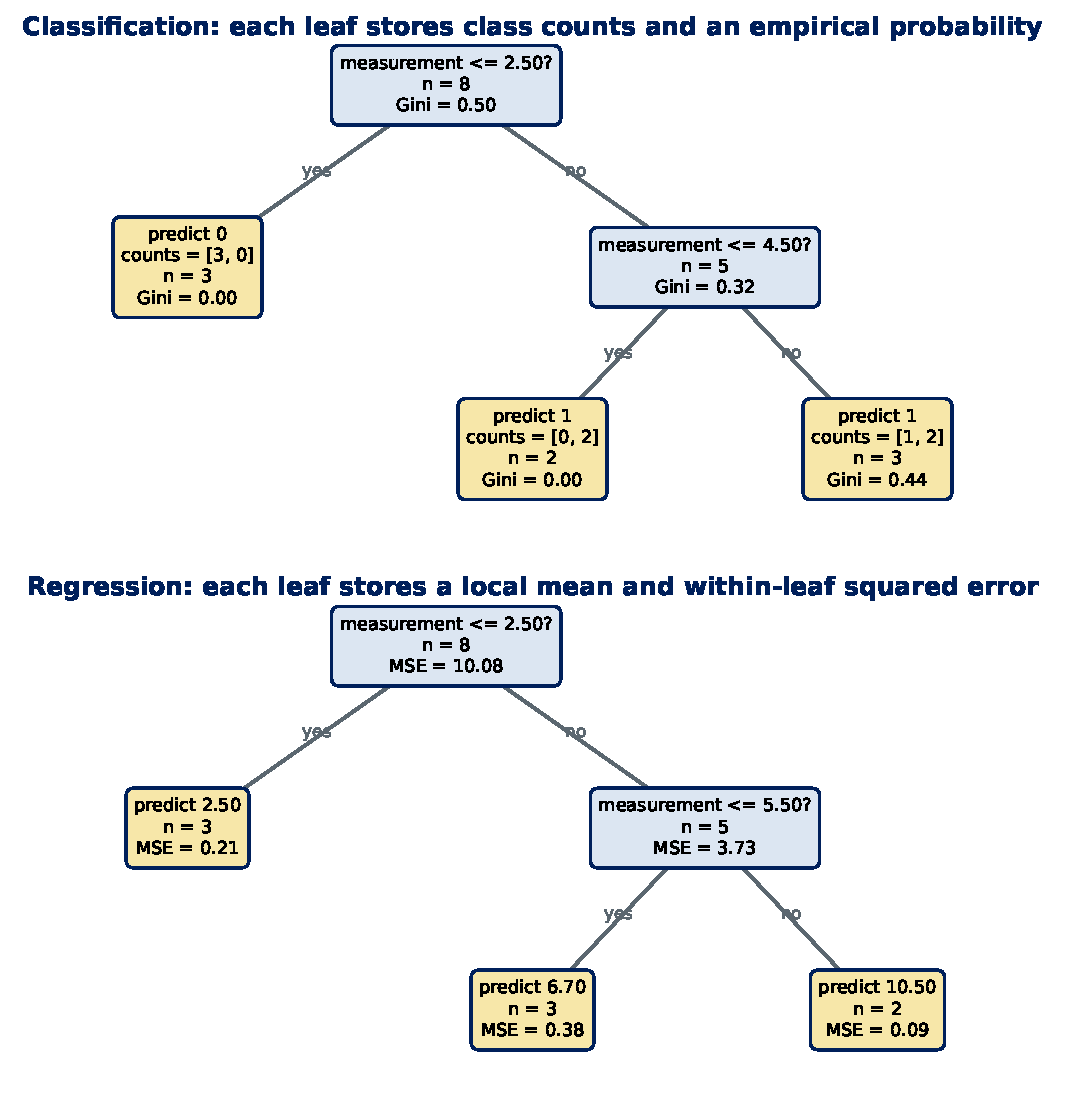
\includegraphics[width=0.96\textwidth]{figures/generated/tree-classification-regression-anatomy.pdf}
  \caption{The anatomy of fitted classification and regression trees. The
  recursive question structure is shared, but node evidence and leaf prediction
  semantics differ. Each diagram describes one fitted artifact, not a causal
  mechanism.}
  \label{fig:tree-anatomy}
\end{figure}

The left panel of Figure~\ref{fig:tree-regression-complexity} contrasts a smooth
data-generating signal with a tree's step function. A tree cannot extrapolate a
trend: outside the training range, it still returns one of its learned leaf
means.

\section{Greedy growth is a computational compromise}

Searching all possible tree structures is combinatorial. Standard algorithms
therefore grow a tree greedily:
\begin{enumerate}
  \item at the current node, sort each feature's observed values;
  \item consider thresholds between distinct adjacent values;
  \item compute the weighted classification impurity or regression SSE;
  \item choose the feature-threshold pair with the largest immediate reduction;
  \item partition the observations and recurse; and
  \item stop when a declared structural or impurity condition is reached.
\end{enumerate}

A locally best split need not appear in the globally best tree. Deterministic
implementations must also define how equal gains, repeated feature values, and
class ties are resolved. Those choices can change structure without materially
changing aggregate performance.

Depth, minimum samples per split, minimum samples per leaf, maximum leaf count,
and minimum impurity decrease constrain growth. These are statistical
regularizers as well as software parameters. A leaf with one regression target
has zero training impurity but is usually a high-variance estimate of its
region's conditional mean.

\section{Pruning trades fit for structural complexity}

An alternative strategy grows a larger tree and prunes it. Cost-complexity
pruning studies
\[
  R_\alpha(T)=R(T)+\alpha|\widetilde T|,
\]
where $R(T)$ is the sum of terminal-node losses and $|\widetilde T|$ is the
number of leaves. Larger $\alpha$ favors smaller trees. Weakest-link pruning
produces a nested sequence of candidate subtrees rather than searching every
possible subtree independently.

The pruning path is estimated from training data. The value of $\alpha$ is a
hyperparameter and belongs to the validation boundary. Choosing the tree with
the smallest test error leaks final evidence into model selection.

\begin{figure}[htbp]
  \centering
  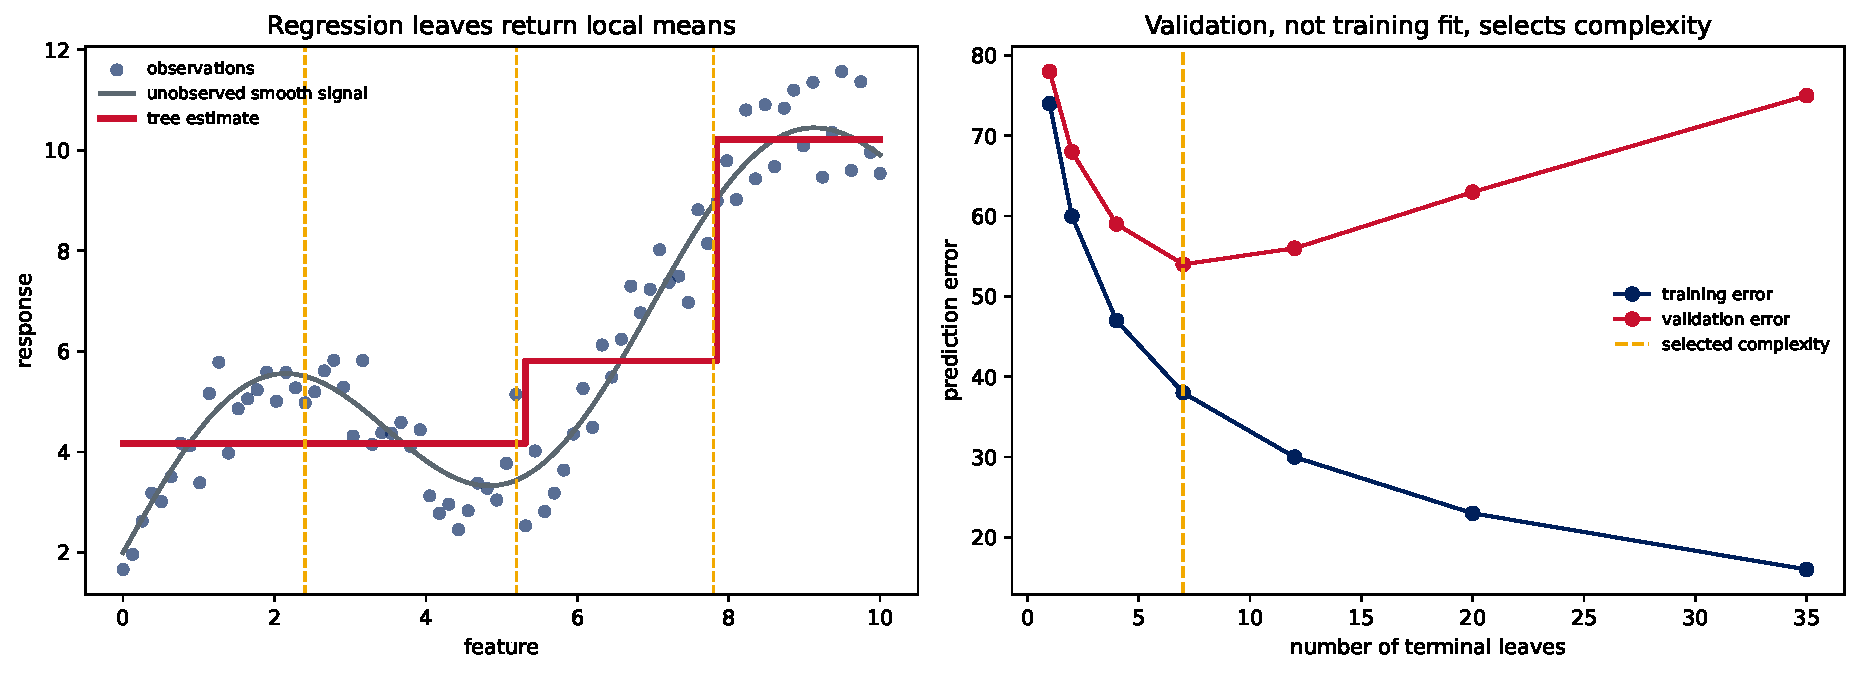
\includegraphics[width=0.96\textwidth]{figures/generated/tree-regression-complexity.pdf}
  \caption{Left: a regression tree approximates a smooth relationship with
  local constants. Right: training error usually decreases as leaves are
  added, while validation error can reach a minimum and then rise. The curves
  are schematic; a real report includes resampling uncertainty.}
  \label{fig:tree-regression-complexity}
\end{figure}

The right panel of Figure~\ref{fig:tree-regression-complexity} illustrates the
bias-variance tradeoff. A one-standard-error rule can prefer a smaller tree
whose validation estimate is statistically indistinguishable from the observed
minimum. Simplicity is not automatically correctness, but unnecessary leaves
increase variance, operational surface area, and explanation burden.

\section{Classification evidence is decision evidence}

The Wisconsin Diagnostic Breast Cancer laboratory uses a versioned SQL table
rather than a hidden loader call. Before fitting, the analysis verifies the
observational unit, target encoding, missingness, duplicate identity, class
support, and feature ranges. The target contract explicitly records that zero
means malignant and one means benign.

Training observations estimate thresholds and leaf proportions. Validation
observations choose criterion, depth, leaf size, and pruning. Test observations
are evaluated once after these choices are frozen. Stratification preserves
class support, but a random split remains an assumption about exchangeability.
Patient, site, batch, or temporal dependence would require grouped or temporal
validation instead.

A professional classification report includes a dummy baseline, class support,
balanced accuracy, class-specific precision and recall, a confusion matrix, and
a probability metric when probabilities are claimed. False negatives and false
positives must be interpreted in the problem's encoding and decision context.
The instructional analysis is not evidence of clinical utility.

\begin{misconceptionbox}
\textbf{Misconception:} a shallow classification tree is objective because its
questions can be read. \textbf{Correction:} feature construction, target
encoding, missingness policy, class support, split criterion, validation design,
pruning, and decision threshold all encode choices. Readability does not
establish stability, fairness, calibration, or causality.
\end{misconceptionbox}

\section{Regression evidence includes residual structure}

The diabetes-progression laboratory compares the fitted tree with a mean
baseline. Mean absolute error measures a typical absolute miss in target units;
root mean squared error emphasizes large misses. Scalar metrics are followed by
predicted-versus-observed and residual-versus-predicted plots. Residual pattern,
heteroscedasticity, and extreme errors can reveal failures hidden by an average.

The dataset contains ten baseline variables and a response measured one year
later, but several feature meanings are incompletely documented. This limits
scientific interpretation. A random split is used as an instructional baseline
because no grouping or time variable is supplied; a serious clinical study
would need a validation design aligned with collection sites, patient
dependence, and intended deployment.

Tree-specific regression checks include:
\begin{itemize}
  \item comparing the prediction range with the observed training response
  range to expose non-extrapolation;
  \item inspecting leaf sample counts and target dispersion;
  \item evaluating inputs immediately below, equal to, and above important
  thresholds;
  \item refitting across resamples to measure root-variable and threshold
  instability; and
  \item monitoring reached-leaf frequencies after release.
\end{itemize}

\section{Instability is a defining property}

A small perturbation can change an early split and therefore the entire
downstream partition. Two trees can have similar predictive performance and
very different structures. Bootstrap refits can compare prediction variation,
root-feature frequency, threshold dispersion, and subgroup error. A displayed
tree is an exact account of one artifact, not necessarily a stable account of
the population.

Feature importance needs the same restraint. Impurity importance allocates
training impurity reduction to split variables. It can favor variables with
many candidate thresholds and distribute credit unreliably among correlated
features. Held-out permutation importance asks how prediction deteriorates
under a particular perturbation; dependent features can make that perturbation
unrealistic. Every interpretation must name the model, population,
perturbation, and uncertainty.

\conceptcheck{Two bootstrap trees achieve nearly identical validation RMSE but
choose different root features. Which claim about predictive performance may
still be supported, and which structural interpretation has become weaker?}

\section{Thresholds, missingness, and schema are contracts}

The conventional numerical rule routes equality left:
$x_j\le t$. A boundary test should include
$\operatorname{nextafter}(t,-\infty)$, $t$, and
$\operatorname{nextafter}(t,+\infty)$. Unit conversion, rounding, or feature
reordering can otherwise change paths silently.

Missingness requires a declared policy: reject, impute inside the fitted
pipeline, learn a default direction, or use a native missing-value mechanism.
Missingness may encode collection behavior that changes after deployment.
Categorical variables likewise need a stable vocabulary and unknown-category
policy.

\begin{professionalbox}
Export the exact feature names and order, units, preprocessing, class ordering,
missing-value policy, library and artifact versions, and decision policy with a
tree. At every release, run analytic split tests, fit-before-predict and invalid
input tests, threshold boundary tests, golden prediction tests, and a
trusted-library differential check on a fixed fixture.
\end{professionalbox}

\section{From notebook experiment to maintained package}

The course implementation places impurity functions, node representation,
classifier, regressor, rule export, tree visualization, and pruning behavior in
\texttt{src/rice\_dsm/ml/trees.py}. The notebooks import that implementation;
they do not maintain private copies. Tests specify hand-computable impurities,
split thresholds, equality routing, probability ordering, local means, pruning,
invalid inputs, and reference-library agreement.

The companion student project follows the same boundary:
\begin{itemize}
  \item \texttt{src/dsm\_project/algorithms/student/trees.py} contains the
  reusable estimator;
  \item \texttt{tests/test\_student\_trees.py} contains analytic, failure,
  boundary, and differential contracts;
  \item \texttt{data/local/} contains private or large data that cannot be
  committed;
  \item \texttt{data/fixtures/} contains a small lawful CI fixture; and
  \item a question-led notebook imports the package and presents data,
  validation, evidence, and limitations.
\end{itemize}

Begin from a clean \texttt{main} branch in the companion template at
\url{https://github.com/RandyRDavila/Data-Science-Machine-Learning-Project-Template}:
\begin{lstlisting}[language=bash,numbers=none]
git switch main
git pull --ff-only
git switch -c YOUR-GITHUB-USERNAME/decision-trees
uv sync --locked
\end{lstlisting}

The implementation sequence is issue first, test first, then analysis:
\begin{enumerate}
  \item open an issue defining the observation, target, split policy, baseline,
  data license, and intended decision;
  \item write hand-computable impurity, leaf-prediction, and threshold-boundary
  tests;
  \item implement one public behavior at a time under \texttt{src/} and register
  it explicitly;
  \item put only lawful, small CI data under \texttt{data/fixtures/};
  \item write a self-contained applied notebook that imports the package; and
  \item run the complete quality gate before opening a pull request.
\end{enumerate}

\begin{lstlisting}[language=bash,numbers=none]
uv run ruff check src tests scripts
uv run pytest -q
git status --short
git add src tests notebooks docs data/fixtures
git commit -m "Add decision-tree case study"
git push -u origin YOUR-GITHUB-USERNAME/decision-trees
\end{lstlisting}

The minimum analytic test suite checks Gini and entropy on known class counts,
the regression leaf mean, a hand-computable best threshold, equality routing to
the left child, class-probability ordering, no-extrapolation behavior, invalid
inputs, prediction before fitting, and agreement with a trusted implementation
under a fixed configuration. Notebook execution in a clean kernel is an
integration test; it is not a substitute for the smaller mathematical tests.

The pull request records the issue, dataset provenance and license,
observational unit, target timing, split policy, baseline, selected metrics,
tests, limitations, and one investigated failure. This is the difference
between demonstrating an algorithm and maintaining a reviewable data-science
artifact.

\begin{workedexample}{a brittle degradation rule}
A depth-three regression tree places resistance change at its root and performs
well on a held-out random split. When evaluation instead holds out later
manufacturing batches, performance falls. Repeated fits also move the root
threshold substantially.

Investigation shows that instrument calibration changed between batches. The
tree learned a separator tied to measurement context. The team retains it as a
baseline, documents threshold instability, adds batch-aware validation, and
rejects causal language about resistance. The failure provides useful evidence
about the data-generating system.
\end{workedexample}

\section{Operational evidence after release}

Before outcomes arrive, monitor schema violations, missingness, feature ranges,
category novelty, reached-leaf distribution, prediction distribution, and
latency. A sudden shift into rarely visited leaves can signal acquisition or
population change. After delayed outcomes arrive, join them to identified
predictions and recompute class-conditional errors or residual metrics by time,
site, and relevant subgroup.

Logs must identify model version, schema version, request or batch identity,
decision policy, and failure category without exposing prohibited sensitive
data. Alerts require a governed response: investigate, mitigate, roll back,
retrain, or document why no action is warranted. Monitoring does not repair a
model; it creates evidence for a decision.

\section{Exercises}
\begin{enumerate}
  \item Compute Gini impurity and entropy for class counts $(6,2,2)$. Then
  compute weighted impurity after a proposed split and state whether impurity
  decreases.
  \item Prove the leaf-mean theorem by completing the square rather than using
  derivatives.
  \item Enumerate every midpoint threshold for feature values
  $(1,2,4,7)$ and responses $(1,2,8,9)$. Identify the regression-stump split.
  \item Construct a classification example where an unweighted average of
  child impurities ranks two splits incorrectly.
  \item Explain why strictly increasing feature rescaling preserves candidate
  partitions but does not prevent preprocessing leakage.
  \item Design threshold tests at $t=0.2$ for equality, adjacent floating-point
  values, missing input, infinity, and a unit-converted input.
  \item Compare two bootstrap trees. Report predictive agreement, root-feature
  frequency, threshold dispersion, and one interpretation that is no longer
  defensible.
  \item Design a validation protocol for repeated measurements from patients
  collected at four hospitals over three years.
  \item Add a classification-tree module and analytic test to the companion
  project. Document class ordering and tie behavior in its NumPy-style
  docstring.
  \item Add a regression-tree analysis on a real dataset. Include a baseline,
  residual plot, pruning evidence, extrapolation test, and dataset card.
  \item Propose a production monitoring panel separating label-free signals
  from metrics that require delayed outcomes.
  \item Review a peer pull request for duplicated notebook logic, test leakage,
  unstable feature order, and unsupported causal language.
\end{enumerate}

\begin{chapterreview}
Classification and regression trees construct piecewise-constant predictions
through greedy recursive partitioning. Classification splits reduce weighted
class impurity; regression splits reduce within-leaf squared error, whose
optimal constant is the leaf mean. Depth, leaf size, impurity constraints, and
cost-complexity pruning regularize the model. Trees capture nonlinear
interactions naturally, but they are discontinuous, non-extrapolating, and
often unstable. Their paths describe one fitted artifact within a declared
schema and validation design; they do not establish causality. Professional
work places reusable code and tests in a package, uses notebooks for evidence,
and monitors the released artifact with explicit operational contracts.
\end{chapterreview}

\begin{notebooklink}
Lecture 14 notebook 00 develops classification trees from Gini and entropy
calculations through clinical decision evidence, pruning, stability, threshold
tests, and project packaging. Lecture 14 notebook 01 derives regression-tree
local means and develops residual, pruning, discontinuity, extrapolation,
stability, interpretation, and monitoring evidence.
\end{notebooklink}
